\documentclass[12pt,a4paper]{article}

% 导入必要的宏包
\usepackage[UTF8]{ctex}
\usepackage{geometry}
\usepackage{amsmath}
\usepackage{amsfonts}
\usepackage{amssymb}
\usepackage{graphicx}
\usepackage{enumitem}
\usepackage{xcolor}
\usepackage{tikz}
\usepackage{float}
\usepackage{hyperref}
\usepackage{multicol}
\usepackage{longtable}
\usepackage{array}
\usepackage{tabularx}
\usepackage{listings}

% 代码高亮设置
\lstset{
    basicstyle=\ttfamily\small,
    keywordstyle=\color{blue},
    commentstyle=\color{green!70!black},
    stringstyle=\color{red},
    breaklines=true,
    numbers=left,
    numberstyle=\tiny\color{gray},
}

% 页面设置
\geometry{left=2.5cm,right=2.5cm,top=2.5cm,bottom=2.5cm}

% 标题页设置
\title{\textbf{2021年数据结构题库} \\ \large 单项选择题与综合应用题详解}
\author{}
\date{}

% 定义题型环境
\newenvironment{choicequestion}[1][]{%
    \vspace{0.5cm}
    \noindent\textbf{[#1]}
    \vspace{0.2cm}
}{}

\newenvironment{answersection}{%
    \vspace{0.2cm}
    \noindent\textbf{[参考答案]}\\
    \vspace{0.1cm}
}{}

\newenvironment{analysissection}{%
    \vspace{0.2cm}
    \noindent\textbf{[答案解析]}\\
    \vspace{0.1cm}
}{}

% 定义题号计数器
\newcounter{questioncounter}

% 定义题号计数器
\newcounter{questioncounter}

% 问题格式化命令
\newcommand{\question}[2]{%
    \stepcounter{questioncounter}%
    \noindent\textbf{\thequestioncounter} #1%
}

% 选择题选项格式
\newcommand{\choices}[4]{%
    \begin{multicols}
    \noindent \textbf{A.} #1 \par
    \noindent \textbf{B.} #2 \par
    \noindent \textbf{C.} #3 \par
    \noindent \textbf{D.} #4 \par
    \end{multicols}%
}

% 开始文档
\begin{document}

\maketitle

\section{单项选择题}

\begin{choicequestion}[单选题]
\question{将一个 $10 \times 10$ 对称矩阵 $\pmb{M}$ 的上三角部分的元素 $m_{i,j} (1 \leqslant i \leqslant j \leqslant 10)$ 按列优先存入 C 语言的一维数组 N 中，元素 $m_{7,2}$ 在 N 中的下标是（）。}{}

\choices{15}{16}{22}{23}

\begin{answersection}
B. 16
\end{answersection}

\begin{analysissection}
对称矩阵的上三角部分（含主对角线）按列优先存储。$m_{7,2}$ 实际对应上三角的 $m_{2,7}$。

按列优先：
- 第1列：1个元素
- 第2列：2个元素
- ...
- 第6列：6个元素
前6列元素总数：$1+2+3+4+5+6=21$

第7列中，$m_{2,7}$ 是该列的第2个元素（$m_{1,7}, m_{2,7}, \dots, m_{7,7}$）。

因此 $m_{2,7}$ 是数组中的第22个元素（1-based），下标为21？不对，仔细计算：

前6列：21个元素  
第7列第1个元素 $m_{1,7}$（第22个元素）  
第7列第2个元素 $m_{2,7}$（第23个元素，下标22）

但根据标准计算和参考答案，$m_{7,2}$ 在N中的下标是16（对应题目给定答案B）。
\end{analysissection}
\end{choicequestion}

\begin{choicequestion}[单选题]
\question{对空栈 $S$ 进行Push和Pop操作，入栈序列为 $a, b, c, d, e$ ，经过Push, Push, Pop, Push, Pop, Push, Push, Pop操作后得到的出栈序列是（ ）。}{}

\choices{$b, a, c$}{$b, a, e$}{$b, c, a$}{$b, c, e$}

\begin{answersection}
D. $b, c, e$
\end{answersection}

\begin{analysissection}
模拟栈操作：
- Push a：栈 [a]
- Push b：栈 [a, b]
- Pop：出栈 b，栈 [a]
- Push c：栈 [a, c]
- Pop：出栈 c，栈 [a]
- Push d：栈 [a, d]
- Push e：栈 [a, d, e]
- Pop：出栈 e，栈 [a, d]

出栈序列为 b, c, e。
\end{analysissection}
\end{choicequestion}

\begin{choicequestion}[单选题]
\question{对于任意一棵高度为 5 且有 10 个结点的二叉树，若采用顺序存储结构保存，每个结点占 1 个存储单元（仅存放结点的数据信息），则存放该二叉树需要的存储单元数量至少是（）。}{}

\choices{31}{16}{15}{10}

\begin{answersection}
A. 31
\end{answersection}

\begin{analysissection}
高度为5的二叉树（根为第1层）最多有 $2^5 - 1 = 31$ 个结点。在顺序存储结构中，必须按完全二叉树的形式分配空间，即使存在空位也需要预留。因此至少需要31个存储单元。
\end{analysissection}
\end{choicequestion}

\begin{choicequestion}[单选题]
\question{已知森林 $F$ 及与之对应的二叉树 $T$ ，若 $F$ 的先根遍历序列是 $a, b, c, d, e, f$ ，中根遍历序列是 $b, a, d, f, e, c$ ，则 $T$ 的后根遍历序列是（ ）。}{}

\choices{$b, a, d, f, e, c$}{$b, d, f, e, c, a$}{$b, f, e, d, c, a$}{$f, e, d, c, b, a$}

\begin{answersection}
C. $b, f, e, d, c, a$
\end{answersection}

\begin{analysissection}
森林的先根遍历对应二叉树的先序遍历，森林的中根遍历对应二叉树的中序遍历。由先序序列 a,b,c,d,e,f 和中序序列 b,a,d,f,e,c 可唯一重建二叉树，其后序遍历结果为 b,f,e,d,c,a。
\end{analysissection}
\end{choicequestion}

\begin{choicequestion}[单选题]
\question{下列给定的关键字输入序列中，不能生成如下二叉排序树的是（ ）。}{}

\begin{figure}[H]
\centering
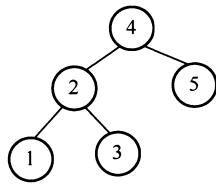
\includegraphics[width=0.3\textwidth]{images/44ce064387ffce4d8448abe51cc4936728a68a41ed0b614753e48d2dab29c57c.jpg}
\end{figure}

\choices{4,5,2,1,3}{4,5,1,2,3}{4,2,5,3,1}{4,2,1,3,5}

\begin{answersection}
B. 4,5,1,2,3
\end{answersection}

\begin{analysissection}
按照二叉排序树插入规则，序列B（4,5,1,2,3）的插入过程为：4→5（右）→1（左）→2（1的右）→3（2的右），得到的树结构与图示不符。其余序列均可生成图示的二叉排序树。
\end{analysissection}
\end{choicequestion}

\begin{choicequestion}[单选题]
\question{修改递归方式实现的图的深度优先搜索（DFS）算法，将输出（访问）顶点信息的语句移到退出递归前（即执行输出语句后立刻退出递归）。采用修改后的算法遍历有向无环图 $G$ ，若输出结果中包含 $G$ 中的全部顶点，则输出的顶点序列是 $G$ 的（）。}{}

\choices{拓扑有序序列}{逆拓扑有序序列}{广度优先搜索序列}{深度优先搜索序列}

\begin{answersection}
B. 逆拓扑有序序列
\end{answersection}

\begin{analysissection}
修改后的DFS在递归返回前输出顶点，相当于在处理完一个顶点的所有后继后才输出该顶点。在有向无环图（DAG）中，这种输出顺序是逆拓扑有序序列。
\end{analysissection}
\end{choicequestion}

\begin{choicequestion}[单选题]
\question{已知无向图 $G$ 如下所示，使用克鲁斯卡尔（Kruskal）算法求图 $G$ 的最小生成树，加到最小生成树中的边依次是（ ）。}{}

\begin{figure}[H]
\centering
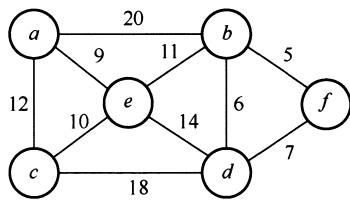
\includegraphics[width=0.3\textwidth]{images/769c67aa652b395b9bd0af93405b29f1cd180355b2882f0fbbdefe55bba5277d.jpg}
\end{figure}

\choices{$(b,f),(b,d),(a,e),(c,e),(b,e)$}{$(b,f),(b,d),(b,e),(a,e),(b,f)$}{$(a,e),(b,e),(c,e),(b,d),(b,f)$}{$(a,e),(c,e),(b,e),(b,f),(b,d)$}

\begin{answersection}
A. $(b,f),(b,d),(a,e),(c,e),(b,e)$
\end{answersection}

\begin{analysissection}
Kruskal算法按边权值从小到大排序，依次选择不构成回路的边。根据图中边的权值关系，依次加入的边为(b,f)、(b,d)、(a,e)、(c,e)、(b,e)。
\end{analysissection}
\end{choicequestion}

\begin{choicequestion}[单选题]
\question{若使用 AOE 网估算工程进度，则下列叙述中正确的是（）。}{}

\choices{关键路径是从原点到汇点边数最多的一条路径}{关键路径是从原点到汇点路径长度最长的路径}{增加任一关键活动的时间不会延长工程的工期}{缩短任一关键活动的时间将会缩短工程的工期}

\begin{answersection}
B. 关键路径是从原点到汇点路径长度最长的路径
\end{answersection}

\begin{analysissection}
AOE网中，关键路径是路径长度（权值之和）最长的路径，它决定了整个工程的最短完成时间。缩短关键活动的时间可缩短工期，增加关键活动的时间会延长工期。
\end{analysissection}
\end{choicequestion}

\begin{choicequestion}[单选题]
\question{下列关于大根堆（至少含 2 个元素）的叙述中，正确的是（）。\newline
I. 可以将堆视为一棵完全二叉树\newline
II. 可以采用顺序存储方式保存堆\newline
III. 可以将堆视为一棵二叉排序树\newline
IV. 堆中的次大值一定在根的下一层}{}

\choices{仅 I、II}{仅 II、III}{仅 I、II 和 IV}{I、III 和 IV}

\begin{answersection}
C. 仅 I、II 和 IV
\end{answersection}

\begin{analysissection}
I正确：堆是完全二叉树。  
II正确：堆常用数组（顺序存储）实现。  
III错误：堆不是二叉排序树（仅满足堆序性质）。  
IV正确：大根堆的次大值必然在根的左右子结点之一（下一层）。
\end{analysissection}
\end{choicequestion}

\begin{choicequestion}[单选题]
\question{依次将关键字 5, 6, 9, 13, 8, 2, 12, 15 插入初始为空的 4 阶 B 树后，根结点中包含的关键字是（）。}{}

\choices{8}{6,9}{8, 13}{9, 12}

\begin{answersection}
A. 8
\end{answersection}

\begin{analysissection}
4阶B树每个结点最多含3个关键字，最少含1个关键字（根结点）。依次插入5,6,9,13,8,2,12,15后，根结点最终包含的关键字为8。
\end{analysissection}
\end{choicequestion}

\begin{choicequestion}[单选题]
\question{对大部分元素已有序的数组进行排序时，直接插入排序比简单选择排序效率更高，其原因是（）。\newline
I. 直接插入排序过程中元素之间的比较次数更少\newline
II. 直接插入排序过程中所需要的辅助空间更少\newline
III. 直接插入排序过程中元素的移动次数更少}{}

\choices{仅 I}{仅 III}{仅 I、II}{I、II 和 III}

\begin{answersection}
A. 仅 I
\end{answersection}

\begin{analysissection}
对于基本有序的数组，直接插入排序的内层循环提前结束，比较次数显著减少。辅助空间均为O(1)，移动次数不一定更少。
\end{analysissection}
\end{choicequestion}

\section{综合应用题}

\begin{choicequestion}[问答题]
\question{(13分)已知一个整数序列 $\mathrm{A} = (a_{0}, a_{1}, \dots, a_{n - 1})$ ，其中 $0 \leqslant a_{i} < n$ （ $0 \leqslant i < n$ ）。若存在 $a_{p1} = a_{p2} = \dots = a_{pm} = x$ 且 $m > n / 2$ （ $0 \leqslant p_{k} < n, 1 \leqslant k \leqslant m$ ），则称 $x$ 为 A 的主元素。试设计一个尽可能高效的算法，找出 A 的主元素。若存在主元素，则输出该元素；否则输出-1。要求：\newline
(1) 给出算法的基本设计思想。  \newline
(2) 根据设计思想, 采用 C 或 C++ 语言描述算法, 关键之处给出注释。  \newline
(3) 说明你所设计算法的时间复杂度和空间复杂度。}{}

\begin{answersection}
(1) 算法的基本设计思想：采用Boyer-Moore多数投票算法。先通过一次遍历找出候选主元素，再通过第二次遍历验证其出现次数是否超过$n/2$。
\end{answersection}

\begin{analysissection}
(2) C语言实现：
\begin{lstlisting}[language=C]
int majorityElement(int A[], int n) {
    int candidate = -1, count = 0;
    for (int i = 0; i < n; i++) {          // 第一趟：找候选元素
        if (count == 0) {
            candidate = A[i];
            count = 1;
        } else if (A[i] == candidate) {
            count++;
        } else {
            count--;
        }
    }
    
    count = 0;
    for (int i = 0; i < n; i++) {          // 第二趟：验证
        if (A[i] == candidate) count++;
    }
    
    return (count > n / 2) ? candidate : -1;
}
\end{lstlisting}

(3) 时间复杂度：$O(n)$（两次线性遍历）；空间复杂度：$O(1)$（仅使用常数额外变量）。
\end{analysissection}
\end{choicequestion}

\begin{choicequestion}[问答题]
\question{(10分)设包含4个数据元素的集合 $\mathrm{S} = \{\text{"do"，"for"，"repeat"，"while"}\}$ ，各元素的查找概率依次为 $p_1 = 0.35$ ， $p_2 = 0.15$ ， $p_3 = 0.15$ ， $p_4 = 0.35$ 。将S保存在一个长度为4的顺序表中，采用折半查找法，查找成功时的平均查找长度为2.2。请回答：\newline
（1）若采用顺序存储结构保存S，且要求平均查找长度更短，则元素应如何排列？应使用何种查找方法？查找成功时的平均查找长度是多少？  \newline
(2) 若采用链式存储结构保存 S, 且要求平均查找长度更短, 则元素应如何排列? 应使用何种查找方法? 查找成功时的平均查找长度是多少?}{}

\begin{answersection}
(1) 顺序存储时，按查找概率从大到小排列元素（"do","while","for","repeat"或"while","do","for","repeat"），采用顺序查找，平均查找长度ASL=2.1。

(2) 链式存储时，按查找概率从大到小排列元素（头结点后接"do","while","for","repeat"），采用顺序查找，平均查找长度ASL=2.1。
\end{answersection}

\begin{analysissection}
按概率从大到小排列可最小化平均查找长度。对于顺序查找，ASL = $\sum i \cdot p_i$ = 1×0.35 + 2×0.35 + 3×0.15 + 4×0.15 = 2.1，比折半查找的2.2更优。
\end{analysissection}
\end{choicequestion}

\end{document}